%===============================================================================
% Autor: Matyáš Sládek
% Rok: 2020
%===============================================================================

\chapter{Přílohy k~extrakci atributů}
\label{prilohy_k_extrakci_atributu}

V~následujícím seznamu jsou uvedeny zvolené hodnoty parametrů extrakční funkce \textit{MusicExtractor} knihovny Essentia.

\begin{itemize}
    \item \textbf{'analysisSampleRate': 44100} - Vzorkovací frekvence skladeb pro analýzu, 44100 Hz (CD kvalita), skladby jsou případně převzorkovány.
    \item \textbf{'endTime': 1e+06} - Jak dlouhý úsek skladby má být analyzován, nastaveno na celou skladbu.
    \item \textbf{'gfccStats': ["mean", "cov", "icov"]} - Jaké statistické funkce použít pro zpracování hodnot gamma tónových kepstrálních koeficientů, nastaveno na průměr, kovarianci a inverzní kovarianci.
    \item \textbf{'loudnessFrameSize': 88200} - Délka okna pro časově-frekvenční analýzu pro odhad hlasitosti, nastaveno na hodnotu 88200 vzorků, což odpovídá úseku dlouhému 2 sekundy. Delší okno je vhodné pro přesnější odhad.
    \item \textbf{'loudnessHopSize': 44100} - Posun okna pro časově-frekvenční analýzu pro odhad hlasitosti, nastaveno na délku poloviny okna, takže se každé okno z~poloviny překrývá z~oknem předchozím.
    \item \textbf{'lowlevelFrameSize': 2048} - Délka okna pro časově-frekvenční analýzu pro výpočet nízko-úrovňových atributů, nastaveno na hodnotu 2048 vzorků, což odpovídá úseku dlouhému 46 milisekund. Kratší okno je vhodné pro přesnější časovou analýzu.
    \item \textbf{'lowlevelHopSize': 1024} - Posun okna pro časově-frekvenční analýzu pro výpočet nízko-úrovňových atributů, nastaveno na délku poloviny okna, takže se každé okno z~poloviny překrývá z~oknem předchozím.
    \item \textbf{'lowlevelSilentFrames': 'noise'} - Zpracování oken neobsahujících zvuk, ponechána výchozí hodnota 'noise' -- doplnění šumem.
    \item \textbf{'lowlevelStats': ["mean", "var", "stdev", "median", "min", "max", "dmean", "dmean2", "dvar", "dvar2"]} - Jaké statistické funkce použít pro zpracování hodnot nízkoúrovňových atributů, nastaveno na průměr, rozptyl, směrodatná odchylka, medián, minimální hodnotu, maximální hodnotu, průměr první derivace, průměr druhé derivace, rozptyl první derivace a rozptyl druhé derivace.
    \item \textbf{'lowlevelWindowType': 'blackmanharris62'} - Typ okénkové funkce pro zpracování oken spektrogramu pro nízkoúrovňové atributy. Nastaveno typ blackmanharris62.
    \item \textbf{'lowlevelZeroPadding': 0} - Odsazení oken pro nízkoúrovňové atributy, nepoužito.
    \item \textbf{'mfccStats': ["mean", "cov", "icov"]} - Jaké statistické funkce použít pro zpracování hodnot Mel-frekvenčních kepstrálních koeficientů, nastaveno na průměr, kovarianci a inverzní kovarianci.
    \item \textbf{'profile': ''} - Profil pro načtení parametrů, nepoužito.
    \item \textbf{'requireMbid': False} - Vyžadovat tag MusicBrainz databáze, nepoužito.
    \item \textbf{'rhythmMaxTempo': 208} - Maximální hodnota tempa, nastaveno na hodnotu 208 úderů za minutu, což by mělo zamezit odhadům tempa ze čtvrtdob a podobně.
    \item \textbf{'rhythmMethod': 'degara'} - Metoda pro odhad tempa, nastaveno na metodu degara.
    \item \textbf{'rhythmMinTempo': 40} - Minimální hodnota tempa, nastaveno na hodnotu 40 úderů za minutu.
    \item \textbf{'rhythmStats': ["mean", "var", "stdev", "median", "min", "max", "dmean", "dmean2", "dvar", "dvar2"]} - Jaké statistické funkce použít pro zpracování hodnot rytmických atributů, nastaveno na průměr, rozptyl, směrodatná odchylka, medián, minimální hodnotu, maximální hodnotu, průměr první derivace, průměr druhé derivace, rozptyl první derivace a rozptyl druhé derivace.
    \item \textbf{'startTime': 0} - Od jakého času začít analýzu, nastaveno na hodnotu 0 sekund.
    \item \textbf{'tonalFrameSize': 4096} - Délka okna pro časově-frekvenční analýzu pro výpočet melodických atributů, nastaveno na hodnotu 4096 vzorků, což odpovídá úseku dlouhému 92 milisekund. Delší okno je vhodné pro přesnější frekvenční odhad.
    \item \textbf{'tonalHopSize': 2048} - Posun okna pro časově-frekvenční analýzu pro výpočet melodických atributů, nastaveno na délku poloviny okna, takže se každé okno z~poloviny překrývá z~oknem předchozím.
    \item \textbf{'tonalSilentFrames': 'noise'} - Zpracování oken neobsahujících zvuk, ponechána výchozí hodnota 'noise' - doplnění šumem.
    \item \textbf{'tonalStats': ["mean", "var", "stdev", "median", "min", "max", "dmean", "dmean2", "dvar", "dvar2"]} - Jaké statistické funkce použít pro zpracování hodnot melodických atributů, nastaveno na průměr, rozptyl, směrodatná odchylka, medián, minimální hodnotu, maximální hodnotu, průměr první derivace, průměr druhé derivace, rozptyl první derivace a rozptyl druhé derivace.
    \item \textbf{'tonalWindowType': 'blackmanharris62'} - Typ okénkové funkce pro zpracování oken spektrogramu pro melodické atributy. Nastaveno typ blackmanharris62.
    \item \textbf{'tonalZeroPadding': 0} - Odsazení oken melodické atributy, nepoužito.
\end{itemize}

\chapter{Přílohy k~výběru klasifikačních algoritmů a jejich parametrů}
\label{prilohy_k_vyberu_klasifikacnich_algoritmu_a_jejich_parametru}

\begin{table}[H]
	\vskip6pt
    \caption{\textbf{Výsledky klasifikace pro výběr parametrů klasifikačních algoritmů na validační sadě}}
    \label{tabulka_classifiers_test_scores}  
    \vskip6pt
	\centering
    \resizebox{\textwidth}{!}{\begin{tabular}{lllllll}
                                                                                  & \multicolumn{2}{l|}{EBD}                & \multicolumn{2}{l|}{FMA}                & \multicolumn{2}{l}{GTZAN} \\
                                                                                  & librosa & \multicolumn{1}{l|}{essentia} & librosa & \multicolumn{1}{l|}{essentia} & librosa     & essentia    \\ \cline{2-7} 
    \multicolumn{1}{l|}{LogisticRegression\_newton-cg}                            & 60.24\% & 87.14\%                       & 44.77\% & 50.47\%                       & 75.63\%     & 84.38\%     \\
    \rowcolor[HTML]{EFEFEF} 
    \multicolumn{1}{l|}{\cellcolor[HTML]{EFEFEF}LogisticRegression\_lbfgs}        & 60.24\% & 87.14\%                       & 44.77\% & 50.39\%                       & 75.63\%     & 84.38\%     \\
    \multicolumn{1}{l|}{LogisticRegression\_liblinear}                            & 58.15\% & 86.70\%                       & 46.88\% & 50.78\%                       & 70.00\%     & 77.50\%     \\
    \rowcolor[HTML]{EFEFEF} 
    \multicolumn{1}{l|}{\cellcolor[HTML]{EFEFEF}LogisticRegression\_sag}          & 61.29\% & 85.95\%                       & 48.05\% & 56.17\%                       & 73.13\%     & 84.38\%     \\
    \multicolumn{1}{l|}{LogisticRegression\_saga}                                 & 62.18\% & 85.95\%                       & 49.61\% & 56.80\%                       & 73.13\%     & 84.38\%     \\
    \rowcolor[HTML]{EFEFEF} 
    \multicolumn{1}{l|}{\cellcolor[HTML]{EFEFEF}KNeighborsClassifier\_ball\_tree} & 41.70\% & 54.11\%                       & 43.98\% & 45.31\%                       & 65.63\%     & 58.13\%     \\
    \multicolumn{1}{l|}{KNeighborsClassifier\_kd\_tree}                           & 41.70\% & 54.11\%                       & 43.98\% & 45.31\%                       & 65.63\%     & 58.13\%     \\
    \rowcolor[HTML]{EFEFEF} 
    \multicolumn{1}{l|}{\cellcolor[HTML]{EFEFEF}KNeighborsClassifier\_brute}      & 41.70\% & 54.11\%                       & 43.98\% & 45.31\%                       & 65.63\%     & 58.13\%     \\
    \multicolumn{1}{l|}{MLPClassifier\_lbfgs}                                     & 59.94\% & 82.96\%                       & 49.69\% & 54.30\%                       & 75.00\%     & 82.50\%     \\
    \rowcolor[HTML]{EFEFEF} 
    \multicolumn{1}{l|}{\cellcolor[HTML]{EFEFEF}MLPClassifier\_sgd}               & 60.99\% & 83.86\%                       & 52.73\% & 51.72\%                       & 74.38\%     & 68.75\%     \\
    \multicolumn{1}{l|}{MLPClassifier\_adam}                                      & 59.94\% & 80.27\%                       & 52.58\% & 57.03\%                       & 76.88\%     & 78.13\%     \\
    \rowcolor[HTML]{EFEFEF} 
    \multicolumn{1}{l|}{\cellcolor[HTML]{EFEFEF}SVC\_linear}                      & 60.24\% & 87.29\%                       & 47.81\% & 52.89\%                       & 75.63\%     & 84.38\%     \\
    \multicolumn{1}{l|}{SVC\_poly}                                                & 38.57\% & 40.36\%                       & 34.06\% & 32.97\%                       & 34.38\%     & 36.88\%     \\
    \rowcolor[HTML]{EFEFEF} 
    \multicolumn{1}{l|}{\cellcolor[HTML]{EFEFEF}SVC\_rbf}                         & 57.70\% & 76.68\%                       & 53.67\% & 57.81\%                       & 68.13\%     & 78.75\%     \\
    \multicolumn{1}{l|}{SVC\_sigmoid}                                             & 46.94\% & 73.84\%                       & 42.34\% & 53.05\%                       & 68.13\%     & 80.00\%    
    \end{tabular}}
\end{table}

\begin{table}[H]
	\vskip6pt
    \caption{\textbf{Doba trénování a klasifikace pro výběr parametrů klasifikačních algoritmů}}
    \label{tabulka_classifiers_test_runtimes}  
    \vskip6pt
	\centering
    \resizebox{\textwidth}{!}{\begin{tabular}{lllllll}
                                                                                  & \multicolumn{2}{l|}{EBD}                & \multicolumn{2}{l|}{FMA}                & \multicolumn{2}{l}{GTZAN} \\
                                                                                  & librosa & \multicolumn{1}{l|}{essentia} & librosa & \multicolumn{1}{l|}{essentia} & librosa     & essentia    \\ \cline{2-7} 
    \multicolumn{1}{l|}{LogisticRegression\_newton-cg}                            & 0:00:07 & 0:00:15                       & 0:00:23 & 0:01:22                       & 0:00:00     & 0:00:02     \\
    \rowcolor[HTML]{EFEFEF} 
    \multicolumn{1}{l|}{\cellcolor[HTML]{EFEFEF}LogisticRegression\_lbfgs}        & 0:00:06 & 0:00:14                       & 0:00:07 & 0:00:25                       & 0:00:00     & 0:00:05     \\
    \multicolumn{1}{l|}{LogisticRegression\_liblinear}                            & 0:00:24 & 0:01:11                       & 0:01:11 & 0:04:39                       & 0:00:02     & 0:00:10     \\
    \rowcolor[HTML]{EFEFEF} 
    \multicolumn{1}{l|}{\cellcolor[HTML]{EFEFEF}LogisticRegression\_sag}          & 0:05:24 & 0:15:23                       & 0:12:37 & 0:31:35                       & 0:00:19     & 0:01:59     \\
    \multicolumn{1}{l|}{LogisticRegression\_saga}                                 & 0:08:24 & 0:22:26                       & 0:17:24 & 0:43:51                       & 0:00:34     & 0:03:01     \\
    \rowcolor[HTML]{EFEFEF} 
    \multicolumn{1}{l|}{\cellcolor[HTML]{EFEFEF}KNeighborsClassifier\_ball\_tree} & 0:00:00 & 0:00:01                       & 0:00:01 & 0:00:05                       & 0:00:00     & 0:00:00     \\
    \multicolumn{1}{l|}{KNeighborsClassifier\_kd\_tree}                           & 0:00:00 & 0:00:02                       & 0:00:02 & 0:00:09                       & 0:00:00     & 0:00:00     \\
    \rowcolor[HTML]{EFEFEF} 
    \multicolumn{1}{l|}{\cellcolor[HTML]{EFEFEF}KNeighborsClassifier\_brute}      & 0:00:00 & 0:00:00                       & 0:00:00 & 0:00:00                       & 0:00:00     & 0:00:00     \\
    \multicolumn{1}{l|}{MLPClassifier\_lbfgs}                                     & 0:00:00 & 0:00:01                       & 0:00:03 & 0:00:08                       & 0:00:00     & 0:00:00     \\
    \rowcolor[HTML]{EFEFEF} 
    \multicolumn{1}{l|}{\cellcolor[HTML]{EFEFEF}MLPClassifier\_sgd}               & 0:00:03 & 0:00:11                       & 0:00:07 & 0:00:18                       & 0:00:00     & 0:00:03     \\
    \multicolumn{1}{l|}{MLPClassifier\_adam}                                      & 0:00:02 & 0:00:05                       & 0:00:06 & 0:00:09                       & 0:00:00     & 0:00:01     \\
    \rowcolor[HTML]{EFEFEF} 
    \multicolumn{1}{l|}{\cellcolor[HTML]{EFEFEF}SVC\_linear}                      & 0:00:08 & 0:00:23                       & 0:00:34 & 0:01:42                       & 0:00:00     & 0:00:01     \\
    \multicolumn{1}{l|}{SVC\_poly}                                                & 0:00:18 & 0:00:59                       & 0:01:00 & 0:03:09                       & 0:00:00     & 0:00:02     \\
    \rowcolor[HTML]{EFEFEF} 
    \multicolumn{1}{l|}{\cellcolor[HTML]{EFEFEF}SVC\_rbf}                         & 0:00:12 & 0:00:39                       & 0:00:43 & 0:02:14                       & 0:00:00     & 0:00:02     \\
    \multicolumn{1}{l|}{SVC\_sigmoid}                                             & 0:00:10 & 0:00:29                       & 0:00:36 & 0:01:54                       & 0:00:00     & 0:00:01    
    \end{tabular}}
\end{table}

\chapter{Přílohy k~selekci atributů}
\label{prilohy_k_selekci_atributu}

\begin{table}[H]
	\vskip6pt
    \caption{\textbf{Doba běhu selekce atributů pomocí dopředné selekce}}
    \label{tabulka_selekce_atributu_forward_selection_runtimes}  
    \vskip6pt
	\centering
    \resizebox{\textwidth}{!}{\begin{tabular}{llllllll}
                                                                            & \multicolumn{2}{l|}{EBD}                 & \multicolumn{2}{l|}{FMA}                 & \multicolumn{2}{l|}{GTZAN}               &                         \\
                                                                            & librosa  & \multicolumn{1}{l|}{essentia} & librosa  & \multicolumn{1}{l|}{essentia} & librosa  & \multicolumn{1}{l|}{essentia} & \multirow{-2}{*}{Total} \\ \cline{2-8} 
        \multicolumn{1}{l|}{LogisticRegression}                             & 00:01:27 & 00:14:28                      & 00:02:13 & 00:36:29                      & 00:00:10 & 00:02:01                      & 00:56:48                \\
        \rowcolor[HTML]{EFEFEF} 
        \multicolumn{1}{l|}{\cellcolor[HTML]{EFEFEF}KneighborsClassifier}   & 00:00:01 & 00:00:48                      & 00:00:08 & 00:01:49                      & 00:00:00 & 00:00:07                      & 00:02:53                \\
        \multicolumn{1}{l|}{MLPClassifier}                                  & 00:06:09 & 00:38:00                      & 00:08:04 & 00:43:26                      & 00:00:57 & 00:06:14                      & 01:42:50                \\
        \rowcolor[HTML]{EFEFEF} 
        \multicolumn{1}{l|}{\cellcolor[HTML]{EFEFEF}DecisionTreeClassifier} & 00:00:19 & 00:02:19                      & 00:03:55 & 00:51:36                      & 00:00:02 & 00:01:04                      & 00:59:15                \\
        \multicolumn{1}{l|}{SVC\_linear}                                    & 00:01:49 & 00:06:08                      & 00:27:39 & 01:12:36                      & 00:00:03 & 00:00:46                      & 01:49:01                \\
        \rowcolor[HTML]{EFEFEF} 
        \multicolumn{1}{l|}{\cellcolor[HTML]{EFEFEF}SVC\_rbf}               & 00:03:38 & 00:19:29                      & 00:07:34 & 04:46:00                      & 00:00:08 & 00:01:56                      & 05:18:45                \\
        \multicolumn{1}{l|}{RandomForestClassifier}                         & 00:00:16 & 00:01:25                      & 00:00:53 & 00:06:18                      & 00:00:03 & 00:00:56                      & 00:09:51                \\
        \rowcolor[HTML]{EFEFEF} 
        \multicolumn{1}{l|}{\cellcolor[HTML]{EFEFEF}XGBClassifier}          & 00:04:13 & 00:26:45                      & 00:11:51 & 02:12:49                      & 00:01:12 & 00:04:50                      & 03:01:40                \\
        \multicolumn{1}{l|}{Total}                                          & 00:17:52 & 01:49:22                      & 01:02:17 & 10:31:03                      & 00:02:35 & 00:17:54                      & 14:01:03               
    \end{tabular}}
\end{table}

\begin{table}[H]
	\vskip6pt
    \caption{\textbf{Doba běhu selekce atributů pomocí zpětné eliminace}}
    \label{tabulka_selekce_atributu_backward_elimination_runtimes}  
    \vskip6pt
	\centering
    \resizebox{\textwidth}{!}{\begin{tabular}{llllllll}
                                                                            & \multicolumn{2}{l|}{EBD}                 & \multicolumn{2}{l|}{FMA}                 & \multicolumn{2}{l|}{GTZAN}               &                         \\
                                                                            & librosa  & \multicolumn{1}{l|}{essentia} & librosa  & \multicolumn{1}{l|}{essentia} & librosa  & \multicolumn{1}{l|}{essentia} & \multirow{-2}{*}{Total} \\ \cline{2-8} 
        \multicolumn{1}{l|}{LogisticRegression}                             & 00:03:33 & 06:23:10                      & 00:03:54 & 04:37:50                      & 00:00:17 & 01:58:18                      & 13:07:02                \\
        \rowcolor[HTML]{EFEFEF} 
        \multicolumn{1}{l|}{\cellcolor[HTML]{EFEFEF}KneighborsClassifier}   & 00:00:07 & 00:05:16                      & 00:00:14 & 00:10:41                      & 00:00:02 & 00:00:42                      & 00:17:02                \\
        \multicolumn{1}{l|}{MLPClassifier}                                  & 00:02:33 & 00:16:24                      & 00:02:37 & 00:52:06                      & 00:00:37 & 00:04:00                      & 01:18:17                \\
        \rowcolor[HTML]{EFEFEF} 
        \multicolumn{1}{l|}{\cellcolor[HTML]{EFEFEF}DecisionTreeClassifier} & 00:01:16 & 00:55:11                      & 00:03:20 & 00:47:59                      & 00:00:15 & 00:04:54                      & 01:52:55                \\
        \multicolumn{1}{l|}{SVC\_linear}                                    & 00:03:27 & 10:45:42                      & 00:21:58 & 13:49:21                      & 00:00:16 & 00:55:39                      & 25:56:23                \\
        \rowcolor[HTML]{EFEFEF} 
        \multicolumn{1}{l|}{\cellcolor[HTML]{EFEFEF}SVC\_rbf}               & 00:06:26 & 07:30:54                      & 00:21:06 & 27:25:49                      & 00:00:25 & 00:42:39                      & 36:07:19                \\
        \multicolumn{1}{l|}{RandomForestClassifier}                         & 00:00:25 & 00:09:50                      & 00:00:39 & 00:12:11                      & 00:00:06 & 00:02:37                      & 00:25:48                \\
        \rowcolor[HTML]{EFEFEF} 
        \multicolumn{1}{l|}{\cellcolor[HTML]{EFEFEF}XGBClassifier}          & 00:10:03 & 05:17:07                      & 00:09:37 & 06:36:02                      & 00:01:24 & 03:34:36                      & 15:48:49                \\
        \multicolumn{1}{l|}{Total}                                          & 00:27:50 & 31:23:34                      & 01:03:25 & 54:31:59                      & 00:03:22 & 07:23:25                      & 94:53:35               
    \end{tabular}}
\end{table}

\begin{table}[H]
	\vskip6pt
    \caption{\textbf{Celková doba běhu trénování a klasifikace na atributech extrahovaných pomocí knihovny Librosa}}
    \label{tabulka_selekce_atributu_librosa_runtimes}  
    \vskip6pt
	\centering
    \resizebox{\textwidth}{!}{\begin{tabular}{llllllllll}
                            &                                                  & LR                              & KNNC                            & MLPC                            & DTC                             & SVCL                            & SVCR                            & RFC                             & XGBC                            \\ \cline{3-10} 
                            & \multicolumn{1}{l|}{All}                         & 0:00:05                         & 0:00:00                         & 0:00:03                         & 0:00:02                         & 0:00:08                         & 0:00:12                         & 0:00:00                         & 0:00:13                         \\
                            & \multicolumn{1}{l|}{\cellcolor[HTML]{EFEFEF}FS}  & \cellcolor[HTML]{EFEFEF}0:00:00 & \cellcolor[HTML]{EFEFEF}0:00:00 & \cellcolor[HTML]{EFEFEF}0:00:12 & \cellcolor[HTML]{EFEFEF}0:00:00 & \cellcolor[HTML]{EFEFEF}0:00:01 & \cellcolor[HTML]{EFEFEF}0:00:02 & \cellcolor[HTML]{EFEFEF}0:00:00 & \cellcolor[HTML]{EFEFEF}0:00:09 \\
    \multirow{-3}{*}{EBD}   & \multicolumn{1}{l|}{BE}                          & 0:00:05                         & 0:00:00                         & 0:00:01                         & 0:00:02                         & 0:00:02                         & 0:00:02                         & 0:00:00                         & 0:00:03                         \\ \cline{1-2}
                            & \multicolumn{1}{l|}{\cellcolor[HTML]{EFEFEF}All} & \cellcolor[HTML]{EFEFEF}0:00:07 & \cellcolor[HTML]{EFEFEF}0:00:00 & \cellcolor[HTML]{EFEFEF}0:00:06 & \cellcolor[HTML]{EFEFEF}0:00:05 & \cellcolor[HTML]{EFEFEF}0:00:33 & \cellcolor[HTML]{EFEFEF}0:00:43 & \cellcolor[HTML]{EFEFEF}0:00:01 & \cellcolor[HTML]{EFEFEF}0:00:22 \\
                            & \multicolumn{1}{l|}{FS}                          & 0:00:01                         & 0:00:00                         & 0:00:04                         & 0:00:04                         & 0:00:20                         & 0:00:07                         & 0:00:01                         & 0:00:15                         \\
    \multirow{-3}{*}{FMA}   & \multicolumn{1}{l|}{\cellcolor[HTML]{EFEFEF}BE}  & \cellcolor[HTML]{EFEFEF}0:00:01 & \cellcolor[HTML]{EFEFEF}0:00:00 & \cellcolor[HTML]{EFEFEF}0:00:04 & \cellcolor[HTML]{EFEFEF}0:00:04 & \cellcolor[HTML]{EFEFEF}0:00:33 & \cellcolor[HTML]{EFEFEF}0:00:09 & \cellcolor[HTML]{EFEFEF}0:00:01 & \cellcolor[HTML]{EFEFEF}0:00:22 \\ \cline{1-2}
                            & \multicolumn{1}{l|}{All}                         & 0:00:00                         & 0:00:00                         & 0:00:00                         & 0:00:00                         & 0:00:00                         & 0:00:00                         & 0:00:00                         & 0:00:04                         \\
                            & \multicolumn{1}{l|}{\cellcolor[HTML]{EFEFEF}FS}  & \cellcolor[HTML]{EFEFEF}0:00:00 & \cellcolor[HTML]{EFEFEF}0:00:00 & \cellcolor[HTML]{EFEFEF}0:00:00 & \cellcolor[HTML]{EFEFEF}0:00:00 & \cellcolor[HTML]{EFEFEF}0:00:00 & \cellcolor[HTML]{EFEFEF}0:00:00 & \cellcolor[HTML]{EFEFEF}0:00:00 & \cellcolor[HTML]{EFEFEF}0:00:01 \\
    \multirow{-3}{*}{GTZAN} & \multicolumn{1}{l|}{BE}                          & 0:00:00                         & 0:00:00                         & 0:00:00                         & 0:00:00                         & 0:00:00                         & 0:00:00                         & 0:00:00                         & 0:00:01                        
    \end{tabular}}
\end{table}

\begin{table}[H]
	\vskip6pt
    \caption{\textbf{Celková doba běhu trénování a klasifikace na atributech extrahovaných pomocí knihovny Essentia}}
    \label{tabulka_selekce_atributu_essentia_runtimes}  
    \vskip6pt
	\centering
    \resizebox{\textwidth}{!}{\begin{tabular}{llllllllll}
                            &                                                  & LR                              & KNNC                            & MLPC                            & DTC                             & SVCL                            & SVCR                            & RFC                             & XGBC                            \\ \cline{3-10} 
                            & \multicolumn{1}{l|}{All}                         & 0:00:14                         & 0:00:00                         & 0:00:05                         & 0:00:07                         & 0:00:23                         & 0:00:39                         & 0:00:01                         & 0:00:40                         \\
                            & \multicolumn{1}{l|}{\cellcolor[HTML]{EFEFEF}FS}  & \cellcolor[HTML]{EFEFEF}0:00:01 & \cellcolor[HTML]{EFEFEF}0:00:00 & \cellcolor[HTML]{EFEFEF}0:00:01 & \cellcolor[HTML]{EFEFEF}0:00:00 & \cellcolor[HTML]{EFEFEF}0:00:00 & \cellcolor[HTML]{EFEFEF}0:00:02 & \cellcolor[HTML]{EFEFEF}0:00:00 & \cellcolor[HTML]{EFEFEF}0:00:03 \\
    \multirow{-3}{*}{EBD}   & \multicolumn{1}{l|}{BE}                          & 0:00:09                         & 0:00:00                         & 0:00:05                         & 0:00:05                         & 0:00:22                         & 0:00:08                         & 0:00:00                         & 0:00:40                         \\ \cline{1-2}
                            & \multicolumn{1}{l|}{\cellcolor[HTML]{EFEFEF}All} & \cellcolor[HTML]{EFEFEF}0:00:25 & \cellcolor[HTML]{EFEFEF}0:00:00 & \cellcolor[HTML]{EFEFEF}0:00:09 & \cellcolor[HTML]{EFEFEF}0:00:17 & \cellcolor[HTML]{EFEFEF}0:01:42 & \cellcolor[HTML]{EFEFEF}0:02:14 & \cellcolor[HTML]{EFEFEF}0:00:02 & \cellcolor[HTML]{EFEFEF}0:01:14 \\
                            & \multicolumn{1}{l|}{FS}                          & 0:00:02                         & 0:00:00                         & 0:00:07                         & 0:00:06                         & 0:00:07                         & 0:00:15                         & 0:00:00                         & 0:00:27                         \\
    \multirow{-3}{*}{FMA}   & \multicolumn{1}{l|}{\cellcolor[HTML]{EFEFEF}BE}  & \cellcolor[HTML]{EFEFEF}0:00:22 & \cellcolor[HTML]{EFEFEF}0:00:00 & \cellcolor[HTML]{EFEFEF}0:00:12 & \cellcolor[HTML]{EFEFEF}0:00:17 & \cellcolor[HTML]{EFEFEF}0:01:28 & \cellcolor[HTML]{EFEFEF}0:01:24 & \cellcolor[HTML]{EFEFEF}0:00:02 & \cellcolor[HTML]{EFEFEF}0:01:14 \\ \cline{1-2}
                            & \multicolumn{1}{l|}{All}                         & 0:00:05                         & 0:00:00                         & 0:00:01                         & 0:00:01                         & 0:00:01                         & 0:00:02                         & 0:00:00                         & 0:00:12                         \\
                            & \multicolumn{1}{l|}{\cellcolor[HTML]{EFEFEF}FS}  & \cellcolor[HTML]{EFEFEF}0:00:00 & \cellcolor[HTML]{EFEFEF}0:00:00 & \cellcolor[HTML]{EFEFEF}0:00:00 & \cellcolor[HTML]{EFEFEF}0:00:00 & \cellcolor[HTML]{EFEFEF}0:00:00 & \cellcolor[HTML]{EFEFEF}0:00:00 & \cellcolor[HTML]{EFEFEF}0:00:00 & \cellcolor[HTML]{EFEFEF}0:00:01 \\
    \multirow{-3}{*}{GTZAN} & \multicolumn{1}{l|}{BE}                          & 0:00:02                         & 0:00:00                         & 0:00:01                         & 0:00:01                         & 0:00:00                         & 0:00:01                         & 0:00:00                         & 0:00:08                        
    \end{tabular}}
\end{table}

\chapter{Přílohy k~optimalizaci parametrů}
\label{prilohy_k_optimalizaci_parametru}

\begin{table}[H]
	\vskip6pt
    \caption{\textbf{Doba běhu optimalizace parametrů na atributech extrahovaných pomocí knihovny Essentia}}
    \label{tabulka_optimalizace_parametru_essentia_optimisation_runtimes}  
    \vskip6pt
	\centering
    \resizebox{\textwidth}{!}{\begin{tabular}{lllllllllll}
                            &                                                  & LR                               & KNNC                             & MLPC                             & DTC                              & SVCL                             & SVCR                             & RFC                              & XGBC                             & Total                            \\ \cline{3-11} 
                            & \multicolumn{1}{l|}{All}                         & 00:01:29                         & 00:00:37                         & 00:35:36                         & 00:29:30                         & 00:02:22                         & 00:48:03                         & 03:11:00                         & 04:44:32                         & 09:53:09                         \\
                            & \multicolumn{1}{l|}{\cellcolor[HTML]{EFEFEF}FS}  & \cellcolor[HTML]{EFEFEF}00:00:15 & \cellcolor[HTML]{EFEFEF}00:00:03 & \cellcolor[HTML]{EFEFEF}00:10:24 & \cellcolor[HTML]{EFEFEF}00:00:39 & \cellcolor[HTML]{EFEFEF}00:00:08 & \cellcolor[HTML]{EFEFEF}00:03:29 & \cellcolor[HTML]{EFEFEF}00:01:57 & \cellcolor[HTML]{EFEFEF}00:21:30 & \cellcolor[HTML]{EFEFEF}00:38:25 \\
    \multirow{-3}{*}{EBD}   & \multicolumn{1}{l|}{BE}                          & 00:01:00                         & 00:00:18                         & 00:22:05                         & 00:15:16                         & 00:02:18                         & 00:11:13                         & 02:19:16                         & 04:57:46                         & 08:09:12                         \\ \cline{1-2}
                            & \multicolumn{1}{l|}{\cellcolor[HTML]{EFEFEF}All} & \cellcolor[HTML]{EFEFEF}00:08:03 & \cellcolor[HTML]{EFEFEF}00:02:13 & \cellcolor[HTML]{EFEFEF}01:07:24 & \cellcolor[HTML]{EFEFEF}00:42:54 & \cellcolor[HTML]{EFEFEF}00:10:22 & \cellcolor[HTML]{EFEFEF}02:33:06 & \cellcolor[HTML]{EFEFEF}09:47:20 & \cellcolor[HTML]{EFEFEF}15:59:44 & \cellcolor[HTML]{EFEFEF}30:31:06 \\
                            & \multicolumn{1}{l|}{FS}                          & 00:09:08                         & 00:00:05                         & 00:23:20                         & 00:11:05                         & 00:15:45                         & 00:18:00                         & 01:26:22                         & 03:17:07                         & 06:00:52                         \\
    \multirow{-3}{*}{FMA}   & \multicolumn{1}{l|}{\cellcolor[HTML]{EFEFEF}BE}  & \cellcolor[HTML]{EFEFEF}00:08:47 & \cellcolor[HTML]{EFEFEF}00:02:11 & \cellcolor[HTML]{EFEFEF}02:45:05 & \cellcolor[HTML]{EFEFEF}00:44:03 & \cellcolor[HTML]{EFEFEF}00:08:54 & \cellcolor[HTML]{EFEFEF}01:35:59 & \cellcolor[HTML]{EFEFEF}14:27:07 & \cellcolor[HTML]{EFEFEF}12:14:05 & \cellcolor[HTML]{EFEFEF}32:06:11 \\ \cline{1-2}
                            & \multicolumn{1}{l|}{All}                         & 00:00:37                         & 00:00:03                         & 00:09:03                         & 00:02:00                         & 00:00:10                         & 00:02:22                         & 00:34:43                         & 01:22:07                         & 02:11:05                         \\
                            & \multicolumn{1}{l|}{\cellcolor[HTML]{EFEFEF}FS}  & \cellcolor[HTML]{EFEFEF}00:00:03 & \cellcolor[HTML]{EFEFEF}00:00:01 & \cellcolor[HTML]{EFEFEF}00:02:24 & \cellcolor[HTML]{EFEFEF}00:00:20 & \cellcolor[HTML]{EFEFEF}00:00:00 & \cellcolor[HTML]{EFEFEF}00:00:15 & \cellcolor[HTML]{EFEFEF}00:01:12 & \cellcolor[HTML]{EFEFEF}00:11:57 & \cellcolor[HTML]{EFEFEF}00:16:12 \\
    \multirow{-3}{*}{GTZAN} & \multicolumn{1}{l|}{BE}                          & 00:00:19                         & 00:00:02                         & 00:24:58                         & 00:01:44                         & 00:00:05                         & 00:01:03                         & 00:22:02                         & 00:42:38                         & 01:32:51                         \\ \cline{1-2}
    \multicolumn{2}{l|}{Total}                                                 & \cellcolor[HTML]{EFEFEF}00:29:41 & \cellcolor[HTML]{EFEFEF}00:05:33 & \cellcolor[HTML]{EFEFEF}06:00:19 & \cellcolor[HTML]{EFEFEF}02:27:31 & \cellcolor[HTML]{EFEFEF}00:40:04 & \cellcolor[HTML]{EFEFEF}05:33:30 & \cellcolor[HTML]{EFEFEF}32:10:59 & \cellcolor[HTML]{EFEFEF}43:51:26 & \cellcolor[HTML]{EFEFEF}91:19:03
    \end{tabular}}
\end{table}

\begin{table}[H]
	\vskip6pt
    \caption{\textbf{Celková doba běhu trénování a klasifikace na atributech extrahovaných pomocí knihovny Essentia po optimalizaci parametrů}}
    \label{tabulka_optimalizace_parametru_essentia_runtimes}  
    \vskip6pt
	\centering
    \resizebox{\textwidth}{!}{\begin{tabular}{llllllllll}
                            &                                                  & LR                              & KNNC                            & MLPC                            & DTC                             & SVCL                            & SVCR                            & RFC                             & XGBC                            \\ \cline{3-10} 
                            & \multicolumn{1}{l|}{All}                         & 0:00:02                         & 0:00:01                         & 0:00:37                         & 0:00:13                         & 0:00:23                         & 0:00:24                         & 0:00:53                         & 0:01:44                         \\
                            & \multicolumn{1}{l|}{\cellcolor[HTML]{EFEFEF}FS}  & \cellcolor[HTML]{EFEFEF}0:00:00 & \cellcolor[HTML]{EFEFEF}0:00:00 & \cellcolor[HTML]{EFEFEF}0:00:01 & \cellcolor[HTML]{EFEFEF}0:00:00 & \cellcolor[HTML]{EFEFEF}0:00:00 & \cellcolor[HTML]{EFEFEF}0:00:02 & \cellcolor[HTML]{EFEFEF}0:00:00 & \cellcolor[HTML]{EFEFEF}0:00:07 \\
    \multirow{-3}{*}{EBD}   & \multicolumn{1}{l|}{BE}                          & 0:00:09                         & 0:00:00                         & 0:00:33                         & 0:00:05                         & 0:00:22                         & 0:00:08                         & 0:01:08                         & 0:01:37                         \\ \cline{1-2}
                            & \multicolumn{1}{l|}{\cellcolor[HTML]{EFEFEF}All} & \cellcolor[HTML]{EFEFEF}0:00:04 & \cellcolor[HTML]{EFEFEF}0:00:07 & \cellcolor[HTML]{EFEFEF}0:00:44 & \cellcolor[HTML]{EFEFEF}0:00:19 & \cellcolor[HTML]{EFEFEF}0:01:47 & \cellcolor[HTML]{EFEFEF}0:01:59 & \cellcolor[HTML]{EFEFEF}0:03:45 & \cellcolor[HTML]{EFEFEF}0:02:27 \\
                            & \multicolumn{1}{l|}{FS}                          & 0:00:02                         & 0:00:00                         & 0:00:04                         & 0:00:03                         & 0:00:07                         & 0:00:15                         & 0:00:24                         & 0:01:38                         \\
    \multirow{-3}{*}{FMA}   & \multicolumn{1}{l|}{\cellcolor[HTML]{EFEFEF}BE}  & \cellcolor[HTML]{EFEFEF}0:00:07 & \cellcolor[HTML]{EFEFEF}0:00:06 & \cellcolor[HTML]{EFEFEF}0:00:34 & \cellcolor[HTML]{EFEFEF}0:00:19 & \cellcolor[HTML]{EFEFEF}0:01:33 & \cellcolor[HTML]{EFEFEF}0:01:24 & \cellcolor[HTML]{EFEFEF}0:04:42 & \cellcolor[HTML]{EFEFEF}0:03:15 \\ \cline{1-2}
                            & \multicolumn{1}{l|}{All}                         & 0:00:02                         & 0:00:00                         & 0:00:08                         & 0:00:01                         & 0:00:01                         & 0:00:02                         & 0:00:09                         & 0:00:15                         \\
                            & \multicolumn{1}{l|}{\cellcolor[HTML]{EFEFEF}FS}  & \cellcolor[HTML]{EFEFEF}0:00:00 & \cellcolor[HTML]{EFEFEF}0:00:00 & \cellcolor[HTML]{EFEFEF}0:00:01 & \cellcolor[HTML]{EFEFEF}0:00:00 & \cellcolor[HTML]{EFEFEF}0:00:00 & \cellcolor[HTML]{EFEFEF}0:00:00 & \cellcolor[HTML]{EFEFEF}0:00:00 & \cellcolor[HTML]{EFEFEF}0:00:01 \\
    \multirow{-3}{*}{GTZAN} & \multicolumn{1}{l|}{BE}                          & 0:00:02                         & 0:00:00                         & 0:00:07                         & 0:00:00                         & 0:00:00                         & 0:00:00                         & 0:00:04                         & 0:00:06                        
    \end{tabular}}
\end{table}

\chapter{Přílohy ke klasifikaci a zhodnocení výsledků}
\label{prilohy_ke_klasifikaci_a_zhodnoceni_vysledku}

\begin{table}[H]
	\vskip6pt
    \caption{\textbf{Celková doba běhu trénování a klasifikace na atributech extrahovaných pomocí knihovny Essentia s~výchozími parametry na testovací sadě}}
    \label{tabulka_essentia_runtimes_default_test}  
    \vskip6pt
	\centering
    \resizebox{\textwidth}{!}{\begin{tabular}{llllllllll}
                            &                                                  & LR                              & KNNC                            & MLPC                            & DTC                             & SVCL                            & SVCR                            & RFC                             & XGBC                            \\ \cline{3-10} 
                            & \multicolumn{1}{l|}{All}                         & 0:00:17                         & 0:00:00                         & 0:00:06                         & 0:00:10                         & 0:00:34                         & 0:00:58                         & 0:00:01                         & 0:00:48                         \\
                            & \multicolumn{1}{l|}{\cellcolor[HTML]{EFEFEF}FS}  & \cellcolor[HTML]{EFEFEF}0:00:01 & \cellcolor[HTML]{EFEFEF}0:00:00 & \cellcolor[HTML]{EFEFEF}0:00:02 & \cellcolor[HTML]{EFEFEF}0:00:00 & \cellcolor[HTML]{EFEFEF}0:00:01 & \cellcolor[HTML]{EFEFEF}0:00:03 & \cellcolor[HTML]{EFEFEF}0:00:00 & \cellcolor[HTML]{EFEFEF}0:00:04 \\
    \multirow{-3}{*}{EBD}   & \multicolumn{1}{l|}{BE}                          & 0:00:11                         & 0:00:00                         & 0:00:06                         & 0:00:06                         & 0:00:33                         & 0:00:12                         & 0:00:01                         & 0:00:48                         \\ \cline{1-2}
                            & \multicolumn{1}{l|}{\cellcolor[HTML]{EFEFEF}All} & \cellcolor[HTML]{EFEFEF}0:00:34 & \cellcolor[HTML]{EFEFEF}0:00:00 & \cellcolor[HTML]{EFEFEF}0:00:14 & \cellcolor[HTML]{EFEFEF}0:00:22 & \cellcolor[HTML]{EFEFEF}0:02:33 & \cellcolor[HTML]{EFEFEF}0:03:22 & \cellcolor[HTML]{EFEFEF}0:00:03 & \cellcolor[HTML]{EFEFEF}0:01:27 \\
                            & \multicolumn{1}{l|}{FS}                          & 0:00:03                         & 0:00:00                         & 0:00:12                         & 0:00:08                         & 0:00:11                         & 0:00:23                         & 0:00:01                         & 0:00:32                         \\
    \multirow{-3}{*}{FMA}   & \multicolumn{1}{l|}{\cellcolor[HTML]{EFEFEF}BE}  & \cellcolor[HTML]{EFEFEF}0:00:32 & \cellcolor[HTML]{EFEFEF}0:00:00 & \cellcolor[HTML]{EFEFEF}0:00:14 & \cellcolor[HTML]{EFEFEF}0:00:21 & \cellcolor[HTML]{EFEFEF}0:02:13 & \cellcolor[HTML]{EFEFEF}0:02:07 & \cellcolor[HTML]{EFEFEF}0:00:03 & \cellcolor[HTML]{EFEFEF}0:01:27 \\ \cline{1-2}
                            & \multicolumn{1}{l|}{All}                         & 0:00:07                         & 0:00:00                         & 0:00:01                         & 0:00:01                         & 0:00:02                         & 0:00:03                         & 0:00:00                         & 0:00:15                         \\
                            & \multicolumn{1}{l|}{\cellcolor[HTML]{EFEFEF}FS}  & \cellcolor[HTML]{EFEFEF}0:00:00 & \cellcolor[HTML]{EFEFEF}0:00:00 & \cellcolor[HTML]{EFEFEF}0:00:00 & \cellcolor[HTML]{EFEFEF}0:00:00 & \cellcolor[HTML]{EFEFEF}0:00:00 & \cellcolor[HTML]{EFEFEF}0:00:00 & \cellcolor[HTML]{EFEFEF}0:00:00 & \cellcolor[HTML]{EFEFEF}0:00:01 \\
    \multirow{-3}{*}{GTZAN} & \multicolumn{1}{l|}{BE}                          & 0:00:02                         & 0:00:00                         & 0:00:01                         & 0:00:01                         & 0:00:01                         & 0:00:01                         & 0:00:00                         & 0:00:10                        
    \end{tabular}}
\end{table}

\begin{table}[H]
	\vskip6pt
    \caption{\textbf{Celková doba běhu trénování a klasifikace na atributech extrahovaných pomocí knihovny Essentia s~optimalizovanými parametry na testovací sadě}}
    \label{tabulka_essentia_runtimes_optimised_test}  
    \vskip6pt
	\centering
    \resizebox{\textwidth}{!}{\begin{tabular}{llllllllll}
                            &                                                  & LR                              & KNNC                            & MLPC                            & DTC                             & SVCL                            & SVCR                            & RFC                             & XGBC                            \\ \cline{3-10} 
                            & \multicolumn{1}{l|}{All}                         & 0:00:04                         & 0:00:02                         & 0:00:45                         & 0:00:18                         & 0:00:34                         & 0:00:35                         & 0:01:05                         & 0:02:07                         \\
                            & \multicolumn{1}{l|}{\cellcolor[HTML]{EFEFEF}FS}  & \cellcolor[HTML]{EFEFEF}0:00:00 & \cellcolor[HTML]{EFEFEF}0:00:00 & \cellcolor[HTML]{EFEFEF}0:00:02 & \cellcolor[HTML]{EFEFEF}0:00:00 & \cellcolor[HTML]{EFEFEF}0:00:01 & \cellcolor[HTML]{EFEFEF}0:00:03 & \cellcolor[HTML]{EFEFEF}0:00:00 & \cellcolor[HTML]{EFEFEF}0:00:09 \\
    \multirow{-3}{*}{EBD}   & \multicolumn{1}{l|}{BE}                          & 0:00:11                         & 0:00:01                         & 0:00:40                         & 0:00:06                         & 0:00:33                         & 0:00:12                         & 0:01:27                         & 0:01:58                         \\ \cline{1-2}
                            & \multicolumn{1}{l|}{\cellcolor[HTML]{EFEFEF}All} & \cellcolor[HTML]{EFEFEF}0:00:06 & \cellcolor[HTML]{EFEFEF}0:00:10 & \cellcolor[HTML]{EFEFEF}0:00:53 & \cellcolor[HTML]{EFEFEF}0:00:26 & \cellcolor[HTML]{EFEFEF}0:02:41 & \cellcolor[HTML]{EFEFEF}0:02:59 & \cellcolor[HTML]{EFEFEF}0:05:11 & \cellcolor[HTML]{EFEFEF}0:02:55 \\
                            & \multicolumn{1}{l|}{FS}                          & 0:00:03                         & 0:00:00                         & 0:00:06                         & 0:00:04                         & 0:00:11                         & 0:00:23                         & 0:00:34                         & 0:02:01                         \\
    \multirow{-3}{*}{FMA}   & \multicolumn{1}{l|}{\cellcolor[HTML]{EFEFEF}BE}  & \cellcolor[HTML]{EFEFEF}0:00:11 & \cellcolor[HTML]{EFEFEF}0:00:10 & \cellcolor[HTML]{EFEFEF}0:00:45 & \cellcolor[HTML]{EFEFEF}0:00:26 & \cellcolor[HTML]{EFEFEF}0:02:20 & \cellcolor[HTML]{EFEFEF}0:02:07 & \cellcolor[HTML]{EFEFEF}0:06:21 & \cellcolor[HTML]{EFEFEF}0:03:49 \\ \cline{1-2}
                            & \multicolumn{1}{l|}{All}                         & 0:00:02                         & 0:00:00                         & 0:00:08                         & 0:00:01                         & 0:00:02                         & 0:00:03                         & 0:00:14                         & 0:00:18                         \\
                            & \multicolumn{1}{l|}{\cellcolor[HTML]{EFEFEF}FS}  & \cellcolor[HTML]{EFEFEF}0:00:00 & \cellcolor[HTML]{EFEFEF}0:00:00 & \cellcolor[HTML]{EFEFEF}0:00:01 & \cellcolor[HTML]{EFEFEF}0:00:00 & \cellcolor[HTML]{EFEFEF}0:00:00 & \cellcolor[HTML]{EFEFEF}0:00:00 & \cellcolor[HTML]{EFEFEF}0:00:00 & \cellcolor[HTML]{EFEFEF}0:00:01 \\
    \multirow{-3}{*}{GTZAN} & \multicolumn{1}{l|}{BE}                          & 0:00:02                         & 0:00:00                         & 0:00:09                         & 0:00:01                         & 0:00:01                         & 0:00:01                         & 0:00:07                         & 0:00:07                        
    \end{tabular}}
\end{table}

\begin{table}[H]
	\vskip6pt
    \caption{\textbf{Tabulka s~podrobnými informacemi o~finální optimalizaci}}
    \label{tabulka_final_optimisation_info}  
    \vskip6pt
	\centering
    \begin{tabular}{lllll}
                                                              &                                                  & MLPC                             & SVCL                             & XGBC                             \\ \cline{3-5} 
                                                              & \multicolumn{1}{l|}{EBD}                         & 02:46:07                         & 00:03:27                         & 26:07:10                         \\
                                                              & \multicolumn{1}{l|}{\cellcolor[HTML]{EFEFEF}FMA} & \cellcolor[HTML]{EFEFEF}07:32:58 & \cellcolor[HTML]{EFEFEF}00:15:15 & \cellcolor[HTML]{EFEFEF}29:48:28 \\
    \multirow{-3}{*}{Doba běhu optimalizace parametrů}        & \multicolumn{1}{l|}{GTZAN}                       & 01:31:48                         & 00:00:14                         & 07:18:35                         \\ \hline
                                                              & \multicolumn{1}{l|}{EBD}                         & 85.89\%                          & 84.57\%                          & 87.56\%                          \\
                                                              & \multicolumn{1}{l|}{\cellcolor[HTML]{EFEFEF}FMA} & \cellcolor[HTML]{EFEFEF}62.81\%  & \cellcolor[HTML]{EFEFEF}60.94\%  & \cellcolor[HTML]{EFEFEF}64.50\%  \\
    \multirow{-3}{*}{Úspěšnost klasifikace na testovací sadě} & \multicolumn{1}{l|}{GTZAN}                       & 82.00\%                          & 82.00\%                          & 83.50\%                          \\ \hline
                                                              & \multicolumn{1}{l|}{EBD}                         & 0:00:37                          & 0:00:35                          & 0:02:50                          \\
                                                              & \multicolumn{1}{l|}{\cellcolor[HTML]{EFEFEF}FMA} & \cellcolor[HTML]{EFEFEF}0:00:44  & \cellcolor[HTML]{EFEFEF}0:02:42  & \cellcolor[HTML]{EFEFEF}0:06:50  \\
    \multirow{-3}{*}{Doba trénování a klasifikace}            & \multicolumn{1}{l|}{GTZAN}                       & 0:00:09                          & 0:00:02                          & 0:00:26                         
    \end{tabular}
\end{table}

\begin{figure*}[h]
    \centering
    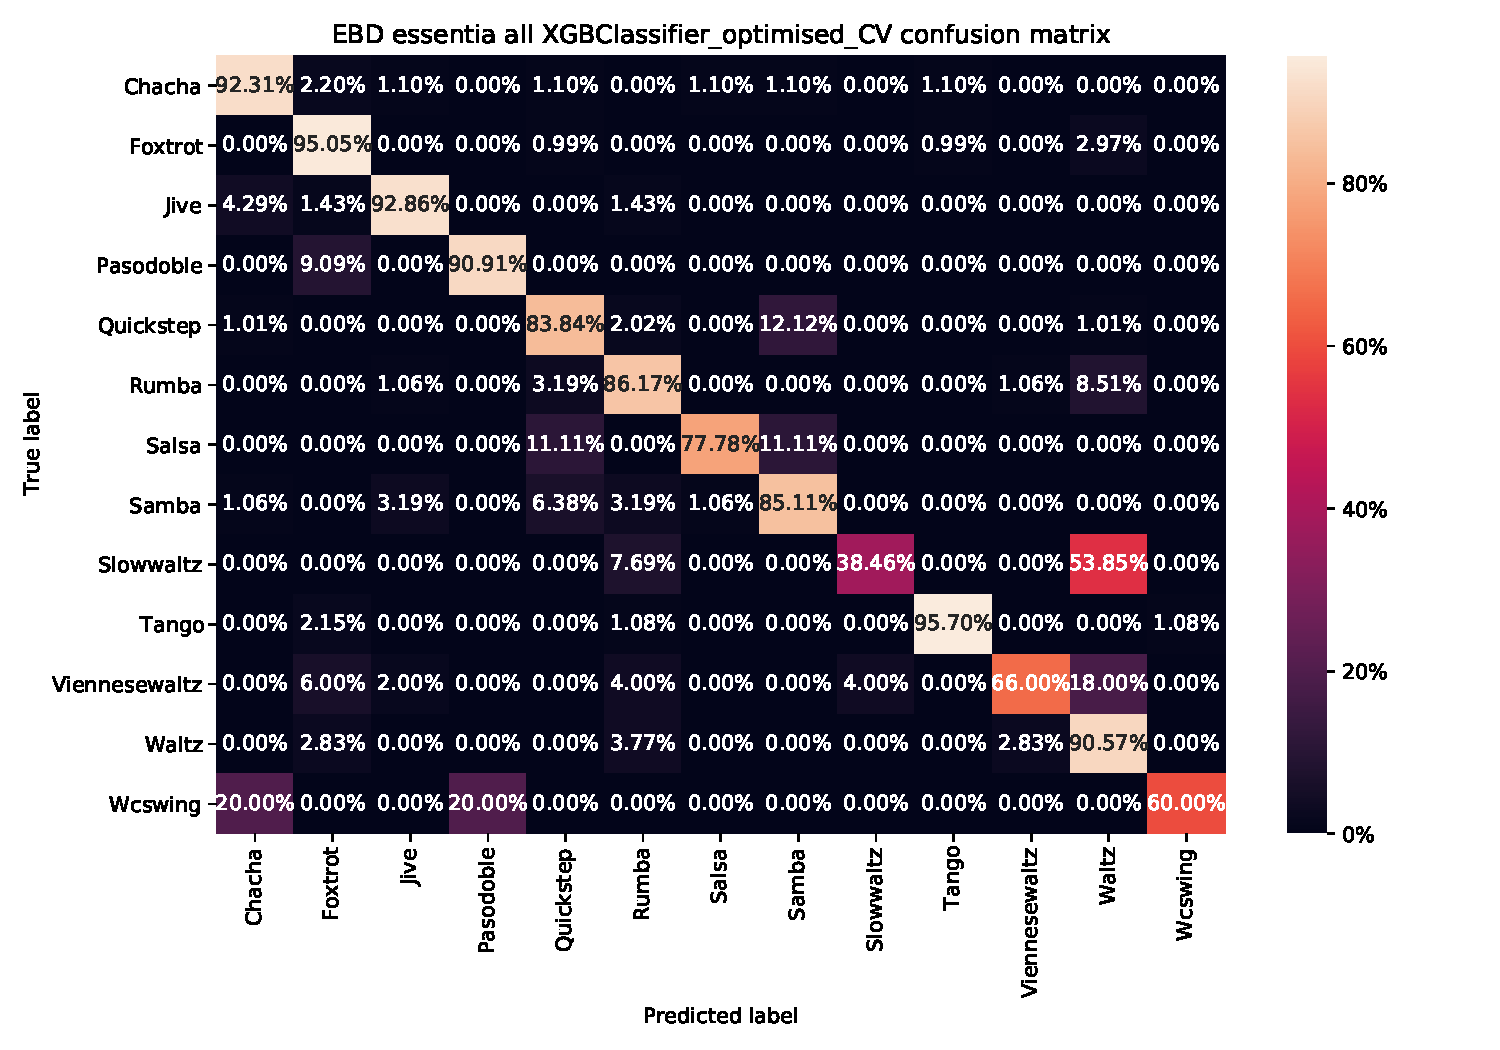
\includegraphics[width=\textwidth]{obrazky/EBD_essentia_all_XGBClassifier_optimised_CV_TS.pdf}
    \caption{\textbf{Matice predikcí nejúspěšnějšího klasifikátoru \textit{XGBClassifier} na datové sadě EBD.}}
    \label{obr_matice_predikce_EBD}
\end{figure*}

\begin{figure*}[h]
    \centering
    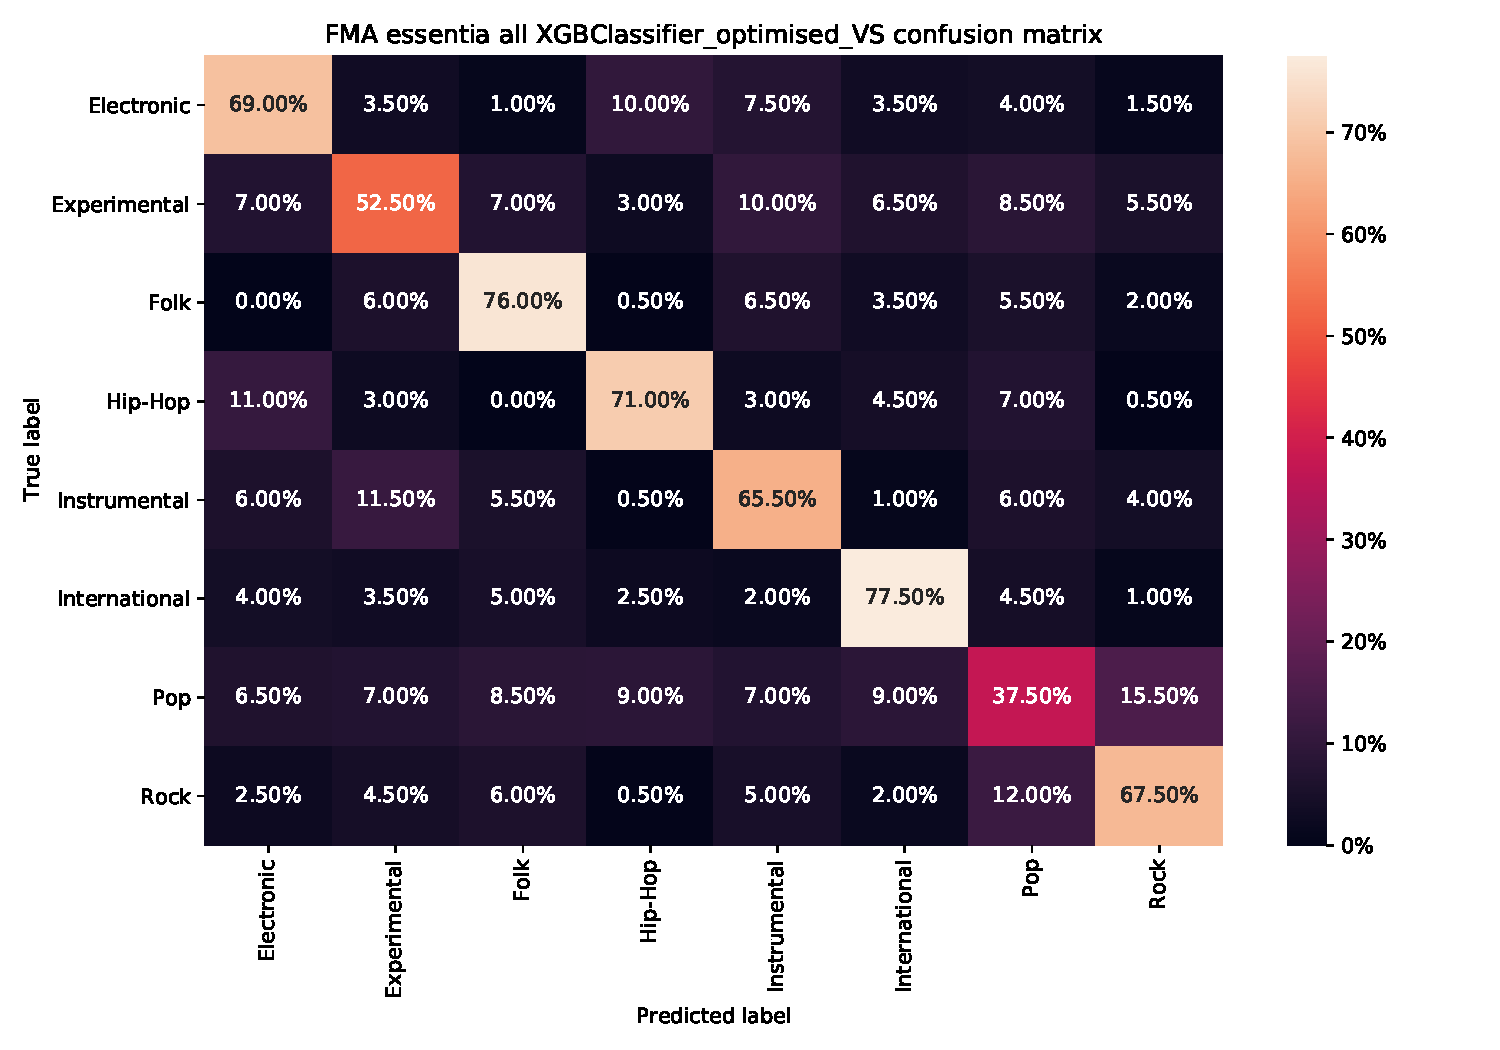
\includegraphics[width=\textwidth]{obrazky/FMA_essentia_all_XGBClassifier_optimised_VS_TS.pdf}
    \caption{\textbf{Matice predikcí nejúspěšnějšího klasifikátoru \textit{XGBClassifier} na datové sadě FMA.}}
    \label{obr_matice_predikce_FMA}
\end{figure*}

\begin{figure*}[h]
    \centering
    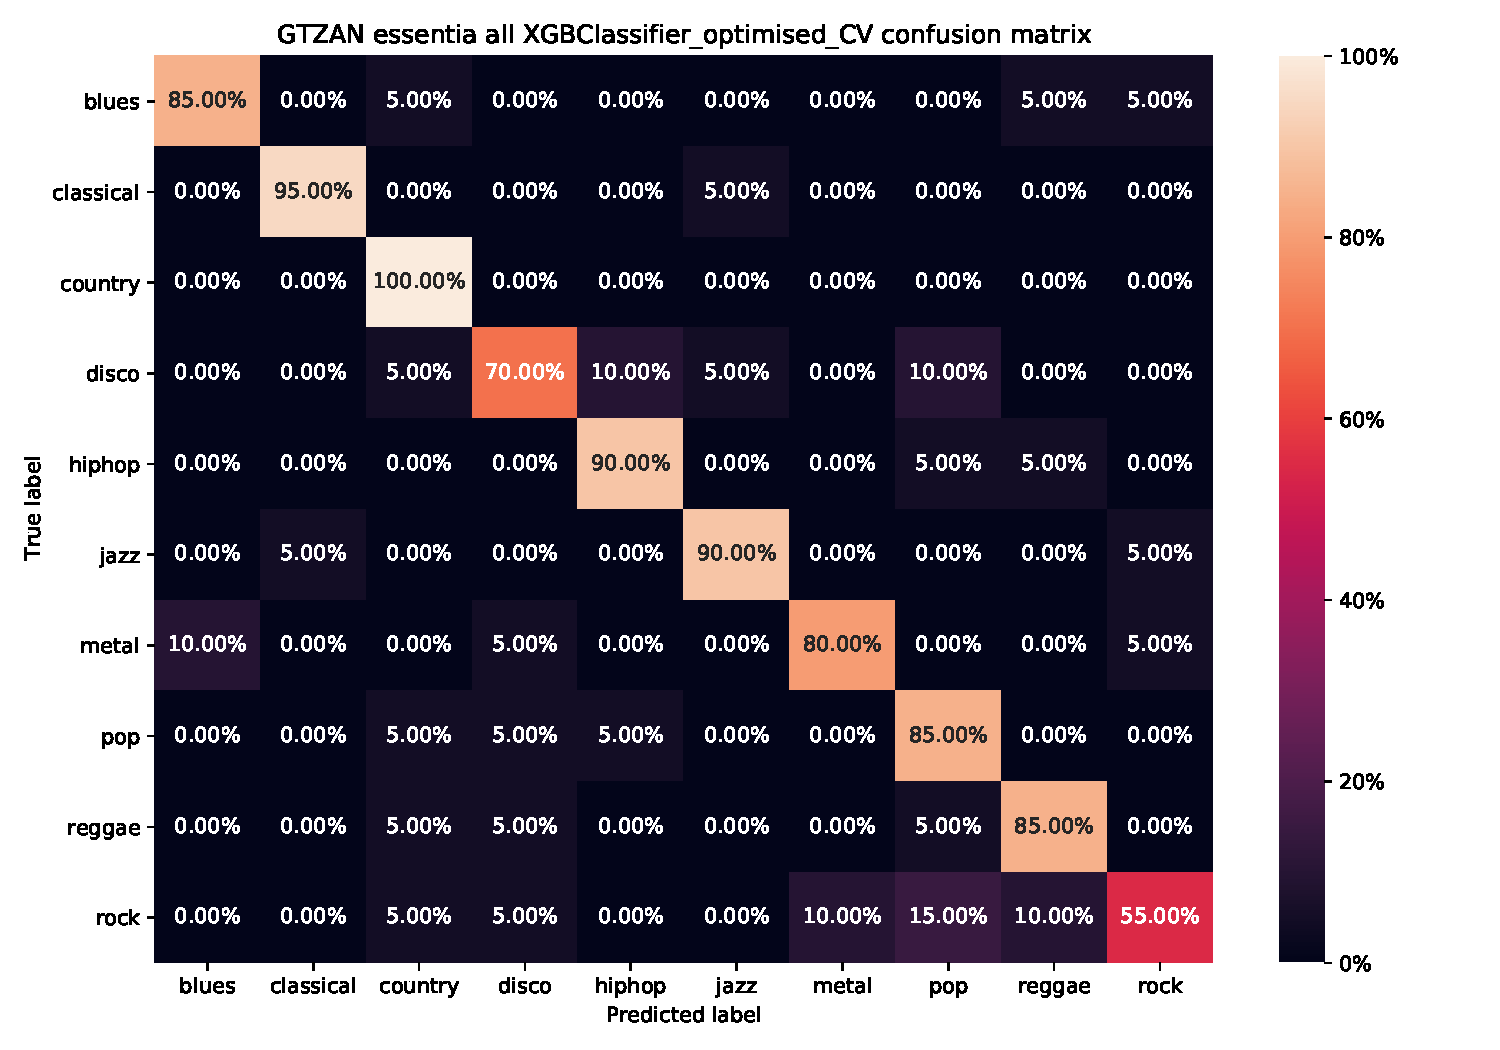
\includegraphics[width=\textwidth]{obrazky/GTZAN_essentia_all_XGBClassifier_optimised_CV_TS.pdf}
    \caption{\textbf{Matice predikcí nejúspěšnějšího klasifikátoru \textit{XGBClassifier} na datové sadě GTZAN.}}
    \label{obr_matice_predikce_GTZAN}
\end{figure*}

\chapter{Obsah přiloženého CD}
\label{obsah_prilozeneho_cd}

\dirtree{%
    .1 /\DTcomment{kořenový adresář přiloženého média}.
    .2 project\DTcomment{adresář obsahující soubory projektu}.
    .3 data\DTcomment{adrasář obsahující testovací skladby}.
    .4 local\_archive\DTcomment{adrasář reprezentující lokální hudební archiv}.
    .5 \dots.
    .3 metadata\DTcomment{adresář obsahující vygenerovaná data}.
    .4 misc\DTcomment{adresář obsahující ostatní soubory}.
    .5 columns\_fix.json\DTcomment{názvy sloupců atributů pro natrénované klasifikátory}.
    .5 feature\_extraction.out\DTcomment{výpis průběhu extrakce atributů}.
    .5 feature\_selection.out\DTcomment{výpis průběhu selekce atributů}.
    .5 optimised\_feature\_sets.json\DTcomment{vybrané podmnožiny atributů}.
    .5 optimised\_hyper\_parameters.json\DTcomment{optimalizované parametry}.
    .4 optuna\_studies\DTcomment{adresář obsahující soubory k~optimalizaci parametrů}.
    .5 EBD\_essentia\_all\_XGBClassifier\_CV.pkl.
    .5 FMA\_essentia\_all\_XGBClassifier\_VS.pkl.
    .5 GTZAN\_essentia\_all\_XGBClassifier\_CV.pkl.
    .4 test\_data\DTcomment{adresář obsahující testovací data}.
    .5 EBD\_genres.csv\DTcomment{žánry testovacích dat EBD}.
    .5 EBD\_X\_test.csv\DTcomment{atributy testovacích dat EBD}.
    .5 FMA\_genres.csv\DTcomment{žánry testovacích dat FMA}.
    .5 FMA\_X\_test.csv\DTcomment{atributy testovacích dat FMA}.
    .5 GTZAN\_genres.csv\DTcomment{žánry testovacích dat GTZAN}.
    .5 GTZAN\_X\_test.csv\DTcomment{atributy testovacích dat GTZAN}.
    .4 track\_genre\_lists\DTcomment{adresář se soubory s~informacemi o~žánrech skladeb}.
    .5 EBD\_track\_genre\_list.csv.
    .5 FMA\_track\_genre\_list.csv.
    .5 GTZAN\_track\_genre\_list.csv.
    .4 trained\_classifiers\DTcomment{adresář obsahující natrénované klasifikátory}.
    .5 EBD\_essentia\_all\_XGBClassifier\_optimised\_CV\_TS.joblib.dat.
    .5 FMA\_essentia\_all\_XGBClassifier\_optimised\_VS\_TS.joblib.dat.
    .5 GTZAN\_essentia\_all\_XGBClassifier\_optimised\_CV\_TS.joblib.dat.
    .3 src\DTcomment{adresář obsahující zdrojové soubory projektu}.
    .4 classification.ipynb\DTcomment{trénování a klasifikace}.
    .4 feature\_extraction.ipynb\DTcomment{extrakce atributů}.
    .4 feature\_selection.ipynb\DTcomment{selekce atributů}.
    .4 hpoptimise\_optuna.ipynb\DTcomment{třída s~funkcemi pro optimalizaci parametrů}.
    .4 images.ipynb\DTcomment{generace obrázků do technické zprávy}.
    .4 local\_archive\_predictions.ipynb\DTcomment{predikce a anotace lokálního archivu}.
    .4 misc.ipynb\DTcomment{funkce pro výpisy výsledků selekce/optimalizace/klasifikace}.
    .4 parameter\_tuning.ipynb\DTcomment{optimalizace parametrů}.
    .4 track\_genre\_list\_creation.ipynb\DTcomment{tvorba souborů s~informacemi o~žánrech}.
    .2 xslade21-latex\DTcomment{adresář obsahující soubory pro generaci technické zprávy}.
    .3 bib-styles\DTcomment{adresář obsahující styly pro latex}.
    .4 \dots.
    .3 obrazky\DTcomment{adresář obsahující obrázky technické zprávy}.
    .4 \dots.
    .3 template-fig\DTcomment{adresář obsahující loga fakulty}.
    .4 \dots.
    .3 fitthesis.cls\DTcomment{latex třída pro technickou zprávu}.
    .3 Makefile\DTcomment{makefile pro vytvoření technické zprávy}.
    .3 xslade21-Klasifikace-hudebnich-souboru.tex.
    .3 xslade21-Klasifikace-hudebnich-souboru-01-kapitoly-chapters.tex.
    .3 xslade21-Klasifikace-hudebnich-souboru-20-literatura-bibliography.bib.
    .3 xslade21-Klasifikace-hudebnich-souboru-30-prilohy-appendices.tex.
    .3 zadani.pdf\DTcomment{zadání projektu}.
    .2 install.sh\DTcomment{skript pro instalaci potřebných knihoven}.
    .2 makefile\DTcomment{makefile pro instalaci Python knihoven (pro install.sh)}.
    .2 Návod-k-instalaci-a-použití.txt\DTcomment{Návod k~instalaci a použití}.
    .2 requirements.txt\DTcomment{seznam potřebných knihoven (pro makefile)}.
    .2 Struktura-obsahu-média.pdf\DTcomment{soubor s~tímto obsahem}.
    .2 xslade21-Klasifikace-hudebnich-souboru.pdf\DTcomment{soubor s~technickou zprávou}.
}